\documentclass[11pt]{article}
\usepackage[a4paper,margin=21mm]{geometry}
\usepackage[T1]{fontenc}
\usepackage{lmodern,amsmath,amssymb,booktabs,array,graphicx,tikz,hyperref,fancyhdr}
\usetikzlibrary{positioning,arrows.meta}
\definecolor{ink}{HTML}{24374A}\definecolor{teal}{HTML}{007F87}\definecolor{rust}{HTML}{BA5730}
\hypersetup{colorlinks=true,urlcolor=teal,linkcolor=teal,pdftitle={Curve25519 representations: research and exact diagnostics}}
\pagestyle{fancy}\fancyhf{}\lhead{\small CURVE25519 / REPRESENTATION RESEARCH}\rhead{\small 17 NOV 2026}\rfoot{\thepage}\setlength{\headheight}{14pt}
\setlength{\emergencystretch}{1em}\setlength{\parindent}{0pt}\setlength{\parskip}{7pt}
\newcommand{\titleline}[2]{{\small\color{teal}\textbf{#1}}\par{\LARGE\color{ink}\textbf{#2}}\par\vspace{3mm}}
\newcommand{\note}[1]{\begin{quote}\color{teal}\textbf{#1}\end{quote}}
\tikzset{box/.style={draw=teal,fill=teal!5,rounded corners,align=center,text width=112mm,minimum height=13mm,font=\small},arr/.style={-{Latex[length=2mm]},thick,draw=ink}}
\begin{document}
\titleline{01 / RESULTS}{What survives a first research pass?}
{\large All five proposed directions, with executable checks and explicit limits.}
\note{The strongest observed benefit is simpler Edwards relation equations. No competitive prime-field attack, asymptotic improvement, or measured runtime advantage was established.}

\begin{tabular}{@{}p{32mm}p{72mm}p{39mm}@{}}\toprule
Direction & Finding & Evidence class\\\midrule
Torsion invariants & $u+1/u$ is a shifted 2-isogeny coordinate; no extra compression on $H/\{\pm1\}$. & Derived; exact checks\\[2mm]
Equation systems & Edwards two-summand equations have 5 monomials in all six symbolic cases; Montgomery has 9. & Exact stage diagnostic\\[2mm]
Factor bases & Coverage changes with coordinate-based selection; no universally best choice in 18 instances. & Exact finite-set census\\[2mm]
Isogenies & Same geometric base transported to the 2-isogenous curve has identical relation multiplicities. & Exact checks; group identity\\[2mm]
Integer lifts & Only $(0,0)$ found on the fixed Curve25519 integer model in $|u|\le10^4$. & Bounded negative result\\\bottomrule
\end{tabular}

\textbf{Additional checks.} All 72 toy scalar-recovery cases passed, with the same public targets also recovered by a rho reference. Twenty-four two-variable reference Gr\"obner computations preserved the checked root sets. One full retained-variable solve hit its fixed correctness-test limit. An independent differential-ladder arithmetic path agreed in 2,895 checks. Elligator 2 was checked over every parameter in each toy field.

\textbf{Scope.} These are CPU correctness tests and exact finite-set diagnostics, not a performance experiment. Toy prime subgroups have orders 11--479. Bases are selected using exhaustive subgroup enumeration, which is explicitly unscalable setup. The scalar-recovery fixtures use $Q=[7]G$; this is a correctness control, not an unseen-target security assessment. No quantum or GPU execution was performed.

\textbf{Prior-work position.} Torsion-aware symmetrization, comparisons among models, composed sparse membership constraints and lifting attacks are established research topics. This bundle connects and checks those ideas; it makes no novelty claim. The research remains limited by source access and is not a comprehensive review through this date.
\newpage
\titleline{02 / A USEFUL IDENTIFICATION}{The torsion invariant is an isogeny coordinate}
For $M_A:v^2=u^3+Au^2+u$ with $A^2\ne4$ and odd characteristic, the point $T=(0,0)$ has order 2. Translation by $T$ acts generically as
\[
 (u,v)\longmapsto(1/u,-v/u^2),\qquad z=u+1/u.
\]
The explicit degree-2 isogeny with kernel $\{\mathcal O,T\}$ is
\[
 \phi(u,v)=\left(u+A+\frac1u,\ v\left(1-\frac1{u^2}\right)\right)=(X,Y),
\]
with target
\[
 M'_A:\quad Y^2=X^3-2AX^2+(A^2-4)X.
\]
Thus $X=z+A$. This identifies two of the proposed research directions rather than providing two independent sources of improvement. At $T$ and $\mathcal O$, the projective extension of $\phi$ has value $\mathcal O$.

\begin{center}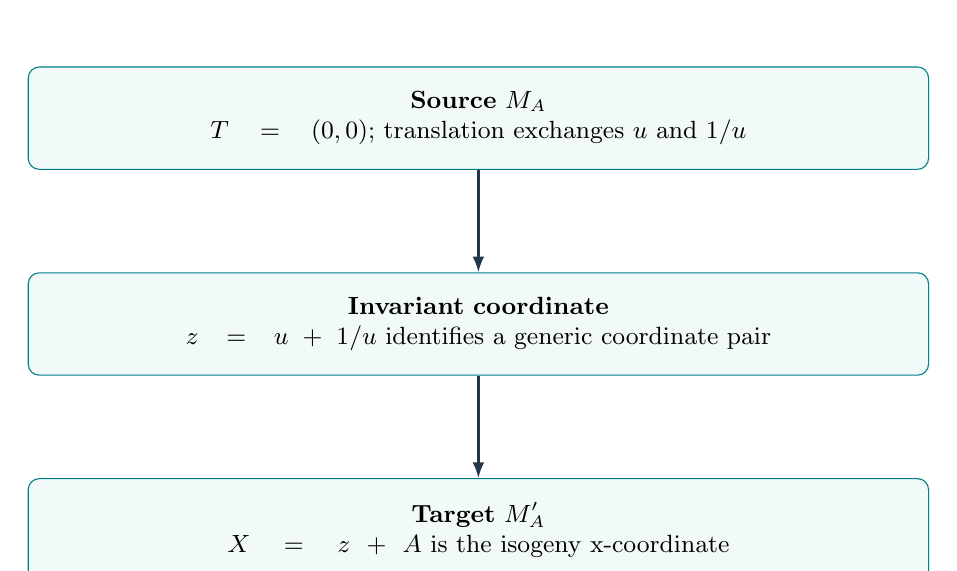
\begin{tikzpicture}[node distance=13mm]
\node[box] (a) {\textbf{Source $M_A$}\\$T=(0,0)$; translation exchanges $u$ and $1/u$};
\node[box,below=of a] (b) {\textbf{Invariant coordinate}\\$z=u+1/u$ identifies a generic coordinate pair};
\node[box,below=of b] (c) {\textbf{Target $M'_A$}\\$X=z+A$ is the isogeny x-coordinate};
\draw[arr] (a)--(b);\draw[arr] (b)--(c);
\end{tikzpicture}\end{center}
This is a symbolic model diagram, not an isogeny-volcano discovery. Exact instance identifiers, source/target coefficients and generators are in \texttt{results.json}. No conductor or volcano level is assigned.

\textbf{Why it does not further compress the prime subgroup.} Let $H$ be an odd-prime-order subgroup. If $z(P)=z(Q)$, their Montgomery coordinates satisfy $u_Q=u_P$ or $u_Q=1/u_P$. Hence generically
\[
 Q\in\{P,-P,P+T,-P+T\}.
\]
But $T\notin H$, so $H\cap(H+T)=\varnothing$. Within $H$, only $Q=\pm P$ remains. Equivalently, $\ker\phi\cap H=\{\mathcal O\}$, so $\phi$ is injective on $H$. All 18 finite censuses confirmed exactly $(r-1)/2$ distinct nonidentity coordinates for each of $u$, Edwards $y$, and $z$.
\newpage
\titleline{03 / EQUATIONS}{Sparsity is real; the algorithmic benefit is open}
Curve25519 has $A=486662$ and $p=2^{255}-19$. Let $c^2=-(A+2)$ and $d=-(A-2)/(A+2)$. Its twisted Edwards model is
\[
 -x^2+y^2=1+dx^2y^2,\quad x=cu/v,\quad y=(u-1)/(u+1).
\]
Writing the same curve in short Weierstrass coordinates uses $X=u+A/3$, $Y=v$. An invertible coordinate change preserves the discrete-log instance and transports any fixed geometric factor base.

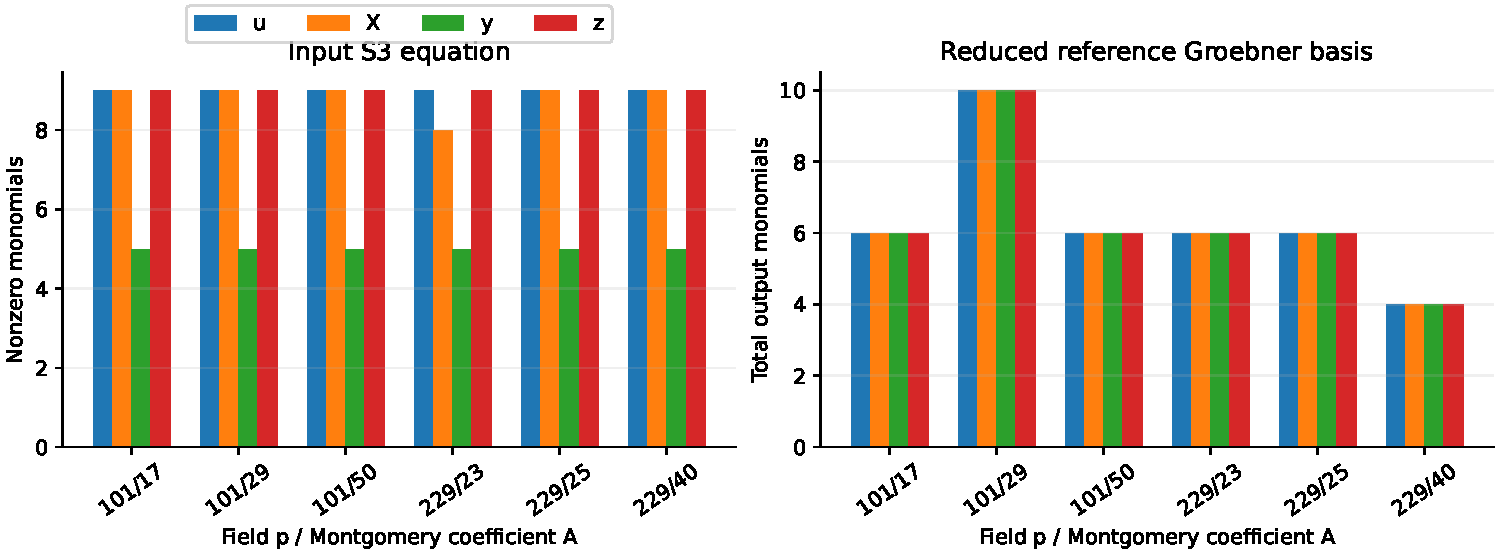
\includegraphics[width=\linewidth]{equations.pdf}
\textbf{Figure.} Six exact $(p,A)$ cases; fixed transported geometric bases and targets. The left panel counts nonzero monomials of a specialized two-summand relation equation. All input equations have total degree 4. The right panel counts monomials in the reduced reference Gr\"obner output, not internal work. Exact counts have no sampling uncertainty; they say nothing about large-field runtime.

\textbf{Retaining products.} For fixed Edwards target $(x_R,y_R)$ and inputs $(x_1,y_1),(x_2,y_2)$, introduce $t=x_1x_2$, $w=y_1y_2$, $h=tw$. The addition constraints become
\[
 x_R(1+dh)=x_1y_2+y_1x_2,\qquad y_R(1-dh)=w+t.
\]
Together with the three product definitions, these are quadratic. The curve constraints can also be split: introduce $t_i=x_i y_i$ and impose $t_i-x_i y_i=0$, $-x_i^2+y_i^2-1-dt_i^2=0$. Factor-base constraints and exceptional-domain handling are still required. More auxiliary variables can offset lower input degrees.

\textbf{What was implemented.} The product constraints were checked on all pairs in each symbolic base, including identity outputs. SymPy computed 24 two-variable Gr\"obner bases and their allowed root sets were checked against the original equations and actual signed point additions. One additional nine-variable, eleven-constraint retained-system solve hit its fixed 45-second check limit in SymPy; no solver correctness outcome was obtained for that case. Its maximum input degree is 3 because of base membership. This negative implementation result reinforces that lower input degrees need not make a system easy. No production F4/F5, SAT, or QUBO performance comparison was run. Input degree and reduced-output size are not solving-degree estimates.
\newpage
\titleline{04 / FACTOR-BASE YIELD}{Different coordinate cuts select different points}
For each toy instance, choose $k=\min(12,\max(3,\lfloor\sqrt r/2\rfloor),(r-1)/2)$ sign classes. Compare the first $k$ classes ordered by $u$, Edwards $y$, or $z$, and a fixed-seed random ordering. The actual signed base contains $2k$ points. Repetition of summands is allowed.

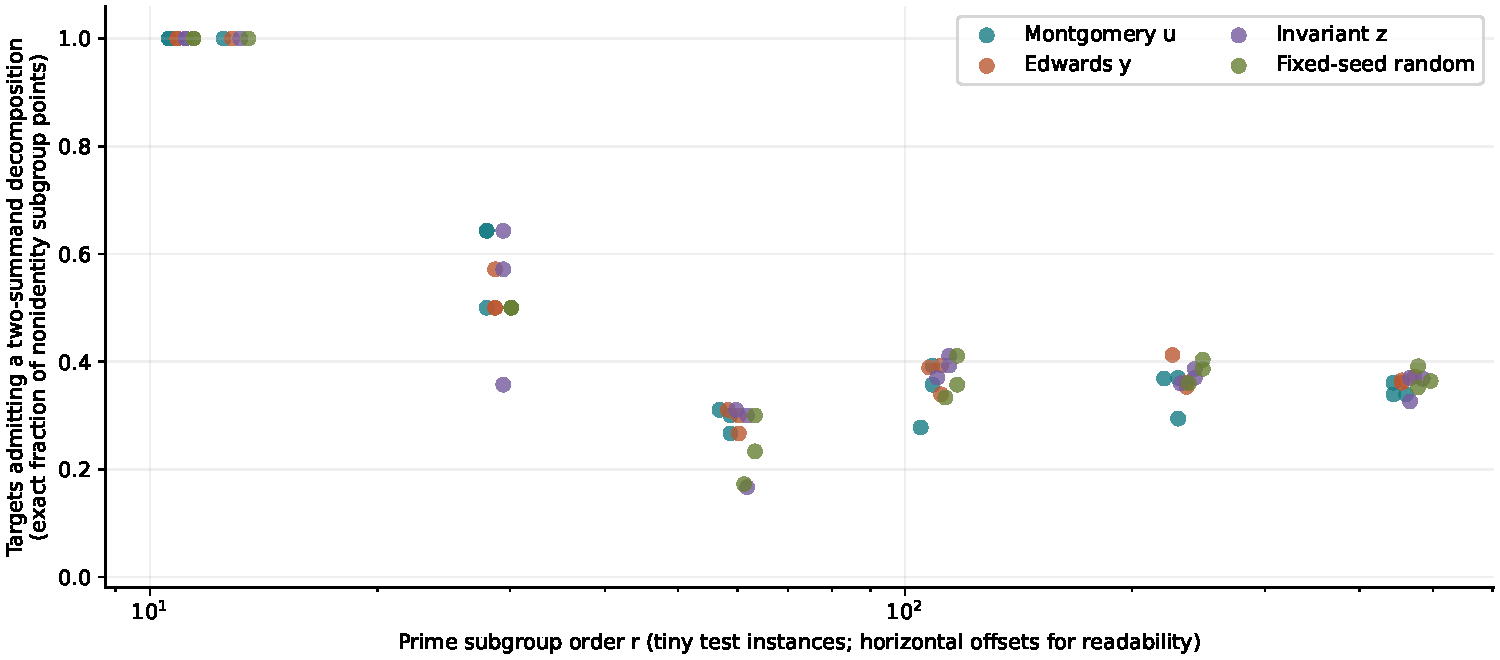
\includegraphics[width=\linewidth]{coverage.pdf}
\textbf{Figure.} Eighteen curves: three per field $p=101,229,461,929,1861,3733$. Each value is an exhaustive fraction over all $r-1$ nonidentity targets, not a sampled success estimate. Horizontal offsets separate marks. There is no sampling error for these finite sets and no asserted uncertainty bound for unseen instances.

\textbf{A useful distinction.} Changing only coordinates while transporting the same points does not change which group relations exist. Selecting points with the smallest values in a new coordinate changes the factor base itself and can change coverage. Those are different experiments.

\textbf{Example.} Over $p=3733$, $A=19$, the prime subgroup has order 461. Ten sign classes give 20 signed points. The counts of nonidentity targets represented as a sum of two base points are 166 ($u$), 168 (Edwards $y$), 150 ($z$), and 180 (the fixed-seed random base). This is one tiny instance, not a ranking of coordinate systems.

\textbf{Controls.} Reversing base enumeration preserved the complete pair-sum histograms. Planted pairs were found and the empty-base check produced no sums. Twelve cofactor-1 curves with coefficient $a=-3$ were also censused: six share the field, six use a field near the torsion-rich subgroup order. They are not fully matched security instances; different field or subgroup orders prevent a clean causal claim about torsion. Their exact parameters remain in the raw data.

\textbf{Result.} No coordinate selection dominates all 18 curves. A different factor base may improve relation yield locally, but it still needs an efficient decomposition solver. Exhaustively enumerating $H$ to select a base is not a scalable attack construction.
\newpage
\titleline{05 / FIELD STRUCTURE}{Sparse membership constraints deserve attention}
A factor base described by $F(u)=\prod_{a\in V}(u-a)=0$ may have a dense, high-degree membership polynomial. An alternative is to choose a multiplicative subgroup of field elements:
\[
 V=\mu_D=\{u\in\mathbb F_p^*:u^D=1\},\qquad D\mid p-1.
\]
If $D=\prod_j q_j$ is smooth, membership can be expressed by a chain of low-degree power maps. Petit--Kosters--Messeng (2016) study this construction and a related auxiliary-isogeny construction. Their paper explicitly does not establish practical superiority to generic attacks.

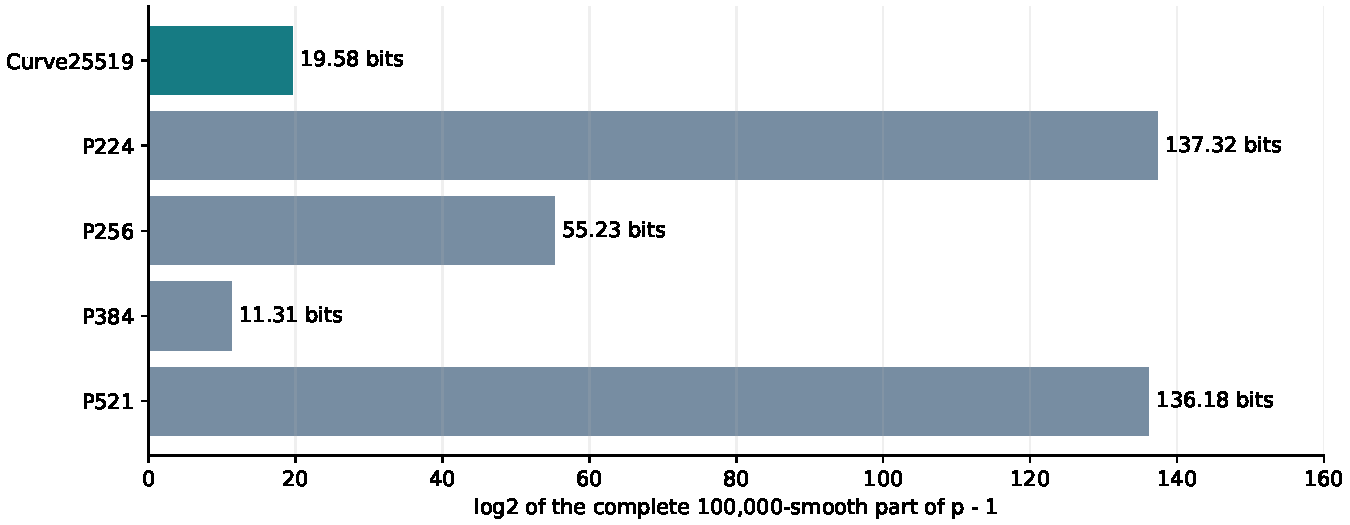
\includegraphics[width=.94\linewidth]{field-structure.pdf}\par
\textbf{Figure.} Exact trial division by every prime through 100,000. The product of those prime powers is fully determined; the residual cofactors were not factored or certified prime. These bit lengths are field-arithmetic descriptors, not security estimates. In particular, $v_2(p-1)=96$ for P-224 and 2 for Curve25519.

\textbf{Combining membership with inversion.} Define Dickson polynomials by $C_0(z)=2$, $C_1(z)=z$, $C_{n+1}(z)=zC_n(z)-C_{n-1}(z)$. Then
\[
 C_D(u+u^{-1})=u^D+u^{-D}=2\qquad(u\in\mu_D).
\]
This gives a concrete way to combine torsion-invariant coordinates and composed membership constraints. Repeated roots, the values $u=\pm1$, lifting and subgroup filtering still matter.

\textbf{Exact check.} For all divisors $D\le64$ of $p-1$ on the 18 instances, 159 structured-base cases were retained and the recurrence identity was checked. Ninety cases had no nonidentity prime-subgroup points at all. Sparse field membership does not guarantee a useful curve factor base. The cases have different actual base sizes and are not a controlled yield comparison against the equal-size bases on page 4.
\newpage
\titleline{06 / ISOGENIES AND ENCODINGS}{Useful transport does not create relations}
\textbf{Target-curve isogeny.} The 2-isogeny on page 2 was checked for curve membership, scalar/addition compatibility and injectivity on every toy prime subgroup. Transporting each of the 72 bases preserved the complete two-summand histogram, including multiplicities. For $\phi$ injective on $H$,
\[
 P_1+P_2=R\quad\Longleftrightarrow\quad
 \phi(P_1)+\phi(P_2)=\phi(R),\qquad P_i,R\in H.
\]
Any benefit must therefore come from cheaper arithmetic, a more tractable equation system, or choosing a \emph{different} target-side base.

\textbf{Auxiliary-curve isogenies are another mechanism.} In the 2016 prime-field construction, an auxiliary curve over the same field supplies an isogeny kernel and composed rational maps defining a coordinate set. It need not be isogenous to the attacked curve. This separates field-level factor-base design from transport of the target discrete log. This bundle checks the target's explicit degree-2 map; it does not implement the paper's general auxiliary-curve search and large composed-map solver.

\textbf{Kummer / x-only representation.} Keeping $u$ already identifies $P$ with $-P$. Addition on this quotient is not an ordinary group law determined by two x-coordinates: differential addition needs additional information. Summation-polynomial roots must be lifted to signed points and replayed as actual relations.

\textbf{Elligator 2.} A field parameter can be mapped to a curve point and then multiplied by the cofactor. The RFC 9380 mapping was checked for every parameter on all 18 toy curves. After cofactor multiplication the outputs lie in $H$, and the code records the number of distinct images. An explicit counterexample to additivity was found on every instance. Encoding inputs are not discrete logarithms and do not convert curve addition into addition of their parameters.

\textbf{Curve25519 itself.} Thirty-two real-parameter point samples passed the coordinate-map, 2-isogeny and torsion-coset tests, with subgroup order also checked. The separate differential ladder validates sampled scalar x-coordinates independently of the affine addition formulas. Finite tests complement the displayed identities; they do not replace proofs, constitute independent-host replay, or assess attack runtime.

\textbf{Full torsion quotient.} Quotienting by a small torsion subgroup disjoint from $H$ remains injective on $H$. Likewise, $[8]$ is a permutation of $H$, although it kills the 2-primary part of the full group. These operations can change representations, but cannot reduce the number of prime-subgroup elements by a factor of eight.
\newpage
\titleline{07 / LIFTS AND EXCEPTIONS}{Two implementation traps, tested explicitly}
\textbf{Fixed integer lift.} We scanned every integer $u$ in $[-10000,10000]$ for
\[
 v^2=u^3+Au^2+u
\]
over the integers, for each of the 18 toy coefficients and $A=486662$. Each candidate square was checked exactly. For the Curve25519 coefficient, only $(0,0)$ was found in this scan. The toy models yielded between one and seven integer points, counting signs.

This is a deliberately narrow diagnostic. It does not enumerate rational points with denominators, alternative coefficient lifts, number-field points, or higher-height points. It establishes neither the rational rank nor an impossibility result for lifting. The classical obstacle is obtaining enough low-height lifts of random finite-field points while maintaining usable group relations; see Galbraith, Chapter 15.9.3.

\textbf{Small coefficients do not preserve small coordinates.} Taking least-residue integer representatives gives a set-theoretic section of reduction, not an elliptic-curve group homomorphism into a fixed rational model. Adjoining a square root separately for each x-coordinate can produce points over varying number fields, but does not supply a common small factor base or an efficient relation algorithm.

\textbf{Affine-chain cancellation.} Every toy instance includes the exact witness
\[
 G+(-G)+[2]G=[2]G.
\]
A chain that stores the first intermediate as an affine pair $(u,v)$ cannot represent $G+(-G)=\mathcal O$. Thus an otherwise correct affine addition chain can omit this decomposition path. The test demonstrates a missing path, not necessarily failure to find every alternative decomposition of the same target.

\begin{center}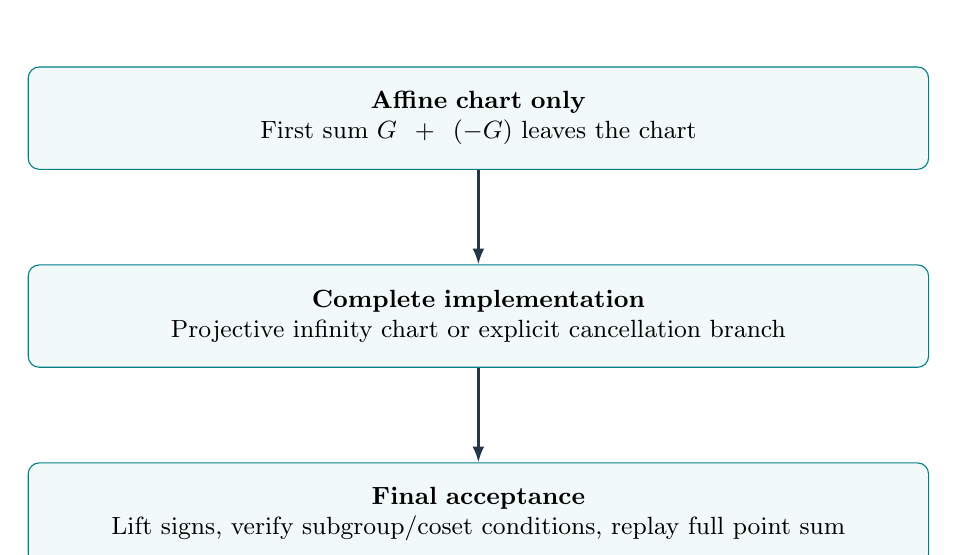
\begin{tikzpicture}[node distance=12mm]
\node[box] (a) {\textbf{Affine chart only}\\First sum $G+(-G)$ leaves the chart};
\node[box,below=of a] (b) {\textbf{Complete implementation}\\Projective infinity chart or explicit cancellation branch};
\node[box,below=of b] (c) {\textbf{Final acceptance}\\Lift signs, verify subgroup/coset conditions, replay full point sum};
\draw[arr] (a)--(b);\draw[arr] (b)--(c);
\end{tikzpicture}\end{center}
Clearing denominators can also admit spurious affine solutions at denominator zeros. Projective coordinates need valid nonzero coordinate tuples and scale handling; low-degree equations alone do not ensure the right solution set.
\newpage
\titleline{08 / IMPLEMENTED PIPELINE}{Scalar recovery works on the toy fixtures}
Each saved base is exercised by a complete correctness pipeline:
\begin{center}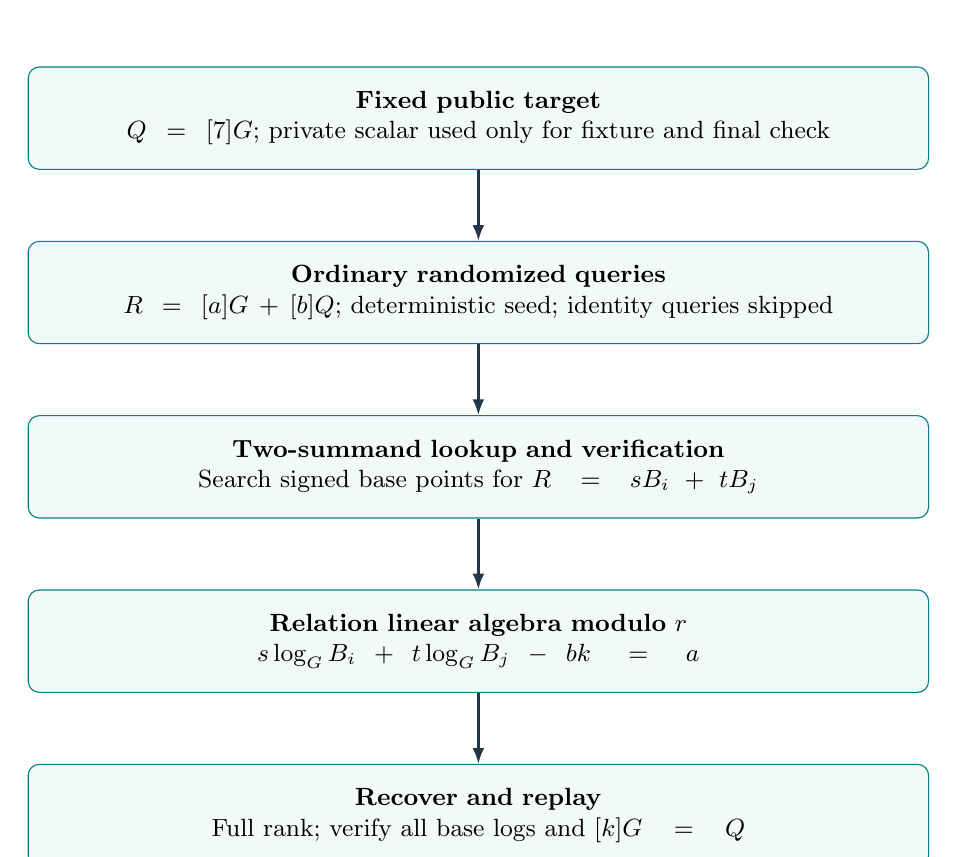
\begin{tikzpicture}[node distance=9mm]
\node[box] (a) {\textbf{Fixed public target}\\$Q=[7]G$; private scalar used only for fixture and final check};
\node[box,below=of a] (b) {\textbf{Ordinary randomized queries}\\$R=[a]G+[b]Q$; deterministic seed; identity queries skipped};
\node[box,below=of b] (c) {\textbf{Two-summand lookup and verification}\\Search signed base points for $R=sB_i+tB_j$};
\node[box,below=of c] (d) {\textbf{Relation linear algebra modulo $r$}\\$s\log_G B_i+t\log_G B_j-bk=a$};
\node[box,below=of d] (e) {\textbf{Recover and replay}\\Full rank; verify all base logs and $[k]G=Q$};
\foreach \a/\b in {a/b,b/c,c/d,d/e}\draw[arr](\a)--(\b);
\end{tikzpicture}\end{center}
\textbf{Result: 72/72 verified.} A three-part Pollard rho implementation recovered the same point on each source instance. The relation solver does not consult a discrete-log table. However, its base-selection stage uses exhaustive toy subgroup enumeration; setup is not scalable. No timing or speedup ratio is reported, and query counts are not a substitute for a charged performance comparison. The decomposition backend is point lookup, not the reference Gr\"obner implementation.

\textbf{What remains open after this pass.} A serious next experiment would implement production polynomial solving for the sparse membership/product systems, retain all exceptional branches, and run fixed unseen-target workloads with full setup, failed-query, lifting, matrix and recovery accounting. It should compare the same geometric base before varying base selection, then compare with optimized same-point rho under matched resources. This bundle supplies correctness fixtures and exact-set baselines, not those performance results.

\textbf{Recommendation.} Prioritize composed sparse membership constraints combined with Edwards product equations, and compare them against the unsplit system on the same base. Torsion quotients are an alternative presentation of that experiment, not a demonstrated extra source of subgroup compression. Keep integer lifting as a lower-priority direction until a concrete common-field, bounded-height relation mechanism is available.
\newpage
\titleline{09 / SOURCES AND REPRODUCTION}{Evidence boundaries and deliverables}
\small
\textbf{Specifications and formulas.} \href{https://www.rfc-editor.org/rfc/rfc7748.html#section-4.1}{RFC 7748} defines the curve and coordinate maps. The \href{https://www.hyperelliptic.org/EFD/g1p/auto-twisted.html}{Explicit-Formulas Database} gives twisted Edwards arithmetic. \href{https://datatracker.ietf.org/doc/html/rfc9380#appendix-F.3}{RFC 9380, Appendix F.3} supplies Elligator 2. These define arithmetic and encodings, not attack claims.

\textbf{Symmetry and model comparisons.} \href{https://doi.org/10.1007/978-3-642-55220-5_3}{Faug\`ere et al. (EUROCRYPT 2014)} exploit small torsion in symmetrized relation equations; the checked abstract reports extension-field results. \href{https://www.jstage.jst.go.jp/article/transfun/E102.A/9/E102.A_1061/_article/-char/en}{Cheng--Kodera--Miyaji (2019)} investigate several models and report empirical differences. Its full PDF required a subscription; this bundle does not claim to replicate their experiments.

\textbf{Prime-field algorithms.} \href{https://christophe.petit.web.ulb.be/files/16PKC_primeECDLP.pdf}{Petit--Kosters--Messeng (PKC 2016)} give composed rational-map factor bases, including smooth $p-1$ and auxiliary-isogeny cases. The author full text was checked, particularly Sections 3.3--3.4 and the conclusion. \href{https://kyushu-u.elsevierpure.com/en/publications/acceleration-of-index-calculus-for-solving-ecdlp-over-prime-field/}{Kudo et al. (CANS 2018)} improve hybrid solving and discuss its limits; the institutional abstract was checked.

\textbf{A conditional negative result.} \href{https://www.degruyterbrill.com/document/doi/10.1515/jmc-2019-0029/html}{Yokoyama--Yasuda--Takahashi--Kogure (2020)} analyze naive summation-polynomial systems. Their method-specific bounds rely on statistical assumptions, including Assumptions 7 and 11 and Conjecture 10 in the relevant analyses. This is not an unconditional lower bound on every elliptic-curve index-calculus method or every solver. The full text and those qualifications were checked.

\textbf{Other directions.} \href{https://reference-global.com/article/10.2478/tmmp-2024-0021?tab=article}{Dzierzkowski--Wro\'nski (2024)} report an Edwards/annealing demonstration over $\mathbb F_{1021}$ with order $4\cdot241$; the publisher abstract was checked, with no quantum execution or performance replication here. \href{https://www.math.auckland.ac.nz/~sgal018/crypto-book/ch15.pdf}{Galbraith, Chapter 15.9.3} discusses lifting obstacles. The local prior note \nolinkurl{representation_join_20261021/report.tex} was checked for its proper-subfield and stage-accounting boundaries.

\textbf{Files.} \texttt{research.py} produces the main census, equations, encodings, lifts and real-curve checks. \texttt{followup.py} adds recovery, Gr\"obner, structured-base and cancellation checks. \texttt{verify.py} performs differential-ladder and artifact cross-checks. \texttt{retained.py} records the bounded full-system solve, including its timeout. \texttt{figures.py} renders vector figures from the JSON. \texttt{PROTOCOL.md} and \texttt{AMENDMENT.md} preserve what was fixed before each set of toy checks; preliminary calculations are explicitly separate. They are standalone scope records, not a certified repository benchmark protocol/export. \texttt{sources.json} records access depth.

\textbf{Reproduce.} Run the three research scripts in that order, then \texttt{retained.py} and \texttt{figures.py}, then run \texttt{pdflatex} \texttt{report.tex} twice. Python dependencies are SymPy, NumPy and Matplotlib. Results contain runtime versions; \texttt{SHA256SUMS} binds the delivered files. No remote service or credentials are needed.

\textbf{Repository status.} This standalone bundle does not change the existing candidate catalog, curve registry, archived factor bases or isogeny graphs. The catalog and prior representation note were checked; none of these bounded diagnostics establishes a new canonical route or performance result that would justify promoting a registry entry.
\end{document}
